\section{Il problema iniziale}
	Prima dell'avvento di Bitcoin era impossibile prescindere dalla mediazione di un sistema centrale per validare dei dati informatici sensibili quanto possono esserlo delle transazioni economiche. \\
	Immaginiamo di dover creare del ``valore digitale" adatto ad essere trasferito in maniera analoga a quanto viene fatto normalmente con il contante. Un primo ingenuo passaggio è quello di associare un valore ad un'entità digitale, sia essa una stringa, un numero, un file o un generico dato, liberamente accessibile oppure in codice. Per loro natura però, i dati digitali sono estremamente facili da replicare: trattandosi in fondo di sequenze di 0 e 1 più o meno lunghe, generarne una copia esatta è un procedimento agevole e sostanzialmente privo di costo. Questo si scontra fortemente con il proposito di creare del valore, dal momento che si ha la necessità di rendere \emph{scarso} il bene. Prendiamo ad esempio il denaro contante: non è accettabile che la stessa cifra sia trasferita due volte dalla stessa persona a due destinatari differenti semplicemente replicando la banconota.
	\begin{figure}[ht]
		\centering
		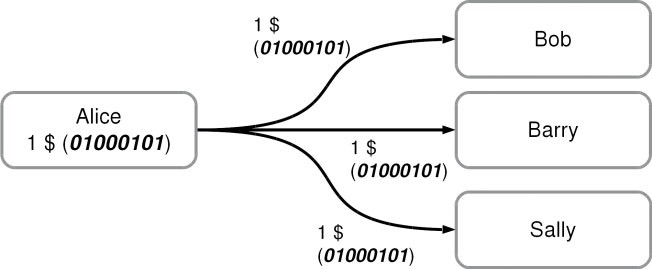
\includegraphics[width=\textwidth]{double_spending_problem.jpg}
		\caption{Double-spending problem, da ``Understanding Bitcoin" \cite{understanding_bitcoin} figura 2.1}
		\label{fig:double-spending_img}
	\end{figure}

	\subsection{Database centralizzato}
		\begin{figure}[ht]
			\centering
			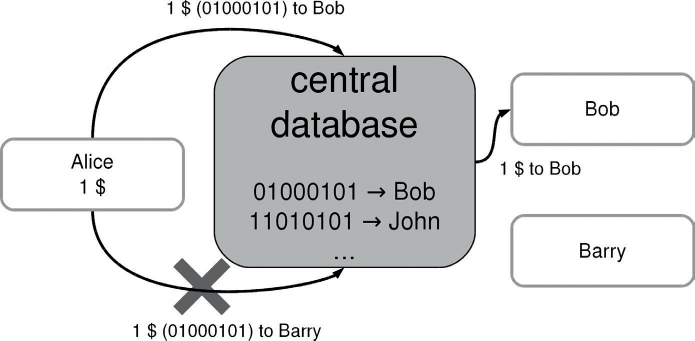
\includegraphics[width=\textwidth]{central_counterparty.png}
			\caption{Central counterparty holding a centralized database, da ``Understanding Bitcoin" \cite{understanding_bitcoin} figura 2.2}
			\label{fig:central_counterparty_img}
		\end{figure}
		La soluzione contro il \emph{double-spending} finora adottata è stata l'affidamento delle transazioni economiche digitali ad un ente esterno fidato (e.g. i sistemi e-banking) che conoscesse le identità degli utenti e potesse verificarne l'effettiva disponibilità economica. È il database centrale che traccia la storia delle transazioni effettuate da ogni utente e prima di autorizzare la successiva verifica che non ci siano incongruenze. \\
		Affidarsi ad un sistema centralizzato risolve il problema, ma porta con sé una serie di criticità. \\
		Prima di tutto la necessità di \emph{trust}, fiducia, nei confronti dell'intermediario centrale: esso infatti ha libero accesso ai dati degli utenti e alla loro storia transazionale, si occupa dell'affidabilità dell'intero sistema, può autorizzare o negare transazioni e bloccare interi utenti. Si tratta di un nodo cruciale per la sicurezza del sistema, un attacco riuscito nei suoi confronti comporterebbe conseguenze disastrose. Inoltre, il database rappresenta un \emph{single point of failure}: abbattere il nodo centrale significa abbattere l'intera rete.

	\subsection{Sistemi distribuiti}
		Un'alternativa ad un sistema controllato da un intermediario centrale è rappresentata da un sistema distribuito decentralizzato. In un sistema distribuito due o più nodi collaborano per svolgere un compito prefissato in maniera trasparente all'utente, che si interfaccia con un'unica piattaforma logica. Emerge la necessità di coordinare i diversi attori: i nodi possono essere onesti e funzionare in modo corretto oppure difettosi, mal funzionanti o maliziosi. Anche se qualche nodo si rivelasse difettoso o la connessione venisse a mancare, un buon sistema distribuito dovrebbe assorbire l'imprevisto e continuare a lavorare senza problemi. La complessità di progettazione di sistemi di questo tipo non è indifferente, è stata area di ricerca fertile per molti anni e lo è tuttora. Un risultato importante è il teorema CAP, che dimostra come non possano coesistere tutte le caratteristiche desiderate in uno stesso sistema.

		\subsubsection{Teorema CAP}\label{sec:teorema_CAP}
			Altrimenti noto come Teorema di Brewer, proposto da Eric Brewer nel 1998 e dimostrato poi da Seth Gilbert e Nancy Lynch nel 2002 \cite{CAP}, il teorema CAP afferma che un qualsiasi sistema distribuito non può garantire simultaneamente le tre seguenti proprietà:
			\begin{itemize}
				\item \textbf{Coerenza (Consistency)} è la proprietà che assicura che tutti i nodi del sistema posseggono la stessa copia aggiornata dei dati;
				\item \textbf{Disponibilità (Availability)} indica che il sistema è attivo, accessibile e pronto a ricevere input e a fornire output corretti nei tempi previsti;
				\item \textbf{Tolleranza di partizione (Partition tolerance)} assicura che anche nel caso un gruppo di nodi crollasse per qualche motivo, il sistema continuerebbe ad operare correttamente.
			\end{itemize}
			\begin{figure}[ht]
				\centering
				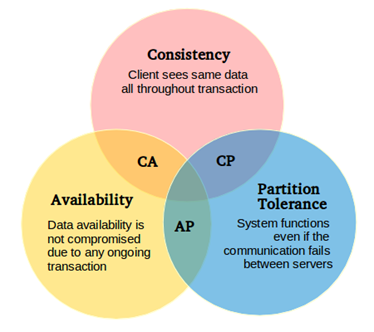
\includegraphics[width=0.7\textwidth]{cap.png}
				\caption{Teorema CAP \cite{cap_diagram}}
				\label{fig:cap}
			\end{figure}

		\subsubsection{Problema dei Generali Bizantini}
			Si tratta di un quesito posto da Leslie Lamport (con Marshall Pease e Robert Shostak) nel 1982 \cite{BGP}, dove un gruppo di generali a capo di diverse sezioni dell'esercito bizantino sta pianificando di attaccare una città. L'unico modo a loro disposizione per comunicare è mediante messaggeri, e hanno bisogno di concordare il momento dell'attacco per vincere. Potrebbero esserci traditori tra di loro, i quali comunicherebbero messaggi discordanti per minare la riuscita dell'operazione: è quindi necessario stabilire un sistema affidabile per raggiungere il consenso sulle tempistiche di attacco. È facile l'analogia con un sistema informatico distribuito in cui i generali siano rappresentati dai nodi e i messaggeri come un'infrastruttura di rete. Una soluzione praticabile del problema dei generali bizantini in un sistema sincrono è stata proposta da Miguel Castro e Barbara Liskov in \emph{Practical Byzantine Fault Tolerance} \cite{PBFT}, mentre Bitcoin è la prima implementazione pratica con la sua soluzione basata sulla Proof-of-Work.

		\subsubsection{Algoritmi di consenso}
			La ricerca sui modi per raggiungere il consenso tra nodi di un sistema distribuito si è sviluppata molto nel periodo successivo all'introduzione di Bitcoin, pertanto sarebbe quantomeno ottimistico fornire un elenco di metodi che volesse essere esaustivo. È possibile tuttavia individuare due categorie principali di algoritmi:
			\begin{itemize}
				\item \textbf{Basati sulla fault-tolerance Bizantina}, si affidano ad un insieme di nodi che si scambiano messaggi firmati. Non richiedono impiego di risorse intensivo, sono affidabili fintanto che $N > 3F$ dove N è il numero di nodi e F è il numero di nodi malevoli;
				\item \textbf{Basati sul riconoscimento di un leader}, mettono i nodi in competizione per essere riconosciuti come leader e il nodo vincitore propone un accordo. Tipicamente richiedono un impiego di risorse considerevole come ``gara" e la sicurezza delle loro applicazioni spesso si basa proprio sulla non convenienza di un tale investimento per un attaccante.
			\end{itemize}

\section{Bitcoin}
	Il 31 ottobre del 2008, uno sconosciuto (o un gruppo) sotto lo pseudonimo di Satoshi Nakamoto annuncia la pubblicazione di un suo paper \cite{nakamoto_bitcoin} in cui presenta un nuovo sistema di moneta elettronica completamente peer-to-peer